%% ICAIF '26 — Paper B (see-market spine)
%% ACM acmart sigconf + anonymous; ≤8 pages; no appendix.
%% Sibling of pdf/icaif26/ (refusal-primary ranking). Differentiated estimand.
\documentclass[sigconf,anonymous]{acmart}

\setcopyright{none}
\acmConference[ICAIF '26]{7th ACM International Conference on AI in Finance}{November 14--17, 2026}{Milan, Italy}
\acmBooktitle{Proceedings of the 7th ACM International Conference on AI in Finance (ICAIF '26)}
\acmDOI{10.1145/XXXXXXX.XXXXXXX}
\acmISBN{978-1-4503-XXXX-X/26/11}
\acmYear{2026}
\copyrightyear{2026}
\settopmatter{printfolios=true,printccs=true,printacmref=true}

\usepackage{booktabs}
\usepackage{array}
\usepackage{amsmath}
\usepackage{graphicx}
\usepackage{listings}
\graphicspath{{figures/}}

\lstset{
  basicstyle=\ttfamily\scriptsize,
  breaklines=true,
  columns=fullflexible,
  frame=single,
  framesep=3pt,
  xleftmargin=0.5em,
  xrightmargin=0.5em,
  aboveskip=4pt,
  belowskip=4pt
}

\makeatletter
\AtEndPreamble{%
  \theoremstyle{acmdefinition}%
  \@ifundefined{assumption}{\newtheorem{assumption}[theorem]{Assumption}}{}%
  \theoremstyle{acmplain}%
  \@ifundefined{remark}{\newtheorem{remark}[theorem]{Remark}}{}%
}
\makeatother

\author{Anonymous Author(s)}
\affiliation{%
  \institution{Anonymous Institution}
  \country{}}
\renewcommand{\shortauthors}{Anon.}

\begin{document}

\title[Seeing Crypto Markets with Public LLMs]{%
  Seeing Crypto Markets with Public LLMs:\texorpdfstring{\\}{ }%
  An Observation Layer that Compiles World Bundles}

\begin{abstract}
\textbf{Purpose.} Public LLMs do not need another trading strategy first; they need to \emph{see} the market.
We build a crypto \emph{observation layer}: an anonymized world-model runtime that compiles asynchronous multi-band evidence into a point-in-time (PIT) \emph{world bundle}---complete, honest, and auditable---for GPT~/DeepSeek~/GLM~/Gemini-class models.
Hard refusal is the safety valve of that layer, not its product definition: when support is thin, a machine-readable flag forces abstention so half-baked context cannot drive decisions.
\textbf{Evidence.} On identical OOS days, a Compiled bundle makes the market legible: grounding recovers ready/missing/tilt at \({\approx}0.97\) vs.\ \({\lesssim}0.23\) under a Raw momentum fragment.
The same layer's quality gate is enforceable across four live vendors (temperature \(0\)): Compiled thin-abstain \(1.0\); Ungated soft judgment on the same content only \({\approx}0.68\); Raw over-trades and loses; Blind refuses with no feed.
This panel is scarce (\(\max\mathrm{WMI}\approx 0.093{<}0.2\)), so Compiled's full refusal is a stress test of the valve, not a claim the layer never opens.
A no-LLM content rule on vintaged tilts beats momentum (\(\Delta\mathrm{CE}{=}0.334\), \(p{=}0.034\)), showing the bundle fields are nonempty.
\textbf{Claim.} Compile so models can see; refuse when they must not act.
\end{abstract}

\begin{CCSXML}
<ccs2012>
 <concept>
  <concept_id>10010147.10010178</concept_id>
  <concept_desc>Computing methodologies~Artificial intelligence</concept_desc>
  <concept_significance>500</concept_significance>
 </concept>
 <concept>
  <concept_id>10010147.10010257</concept_id>
  <concept_desc>Computing methodologies~Machine learning</concept_desc>
  <concept_significance>300</concept_significance>
 </concept>
 <concept>
  <concept_id>10010405.10010455</concept_id>
  <concept_desc>Applied computing~Economics</concept_desc>
  <concept_significance>300</concept_significance>
 </concept>
</ccs2012>
\end{CCSXML}

\ccsdesc[500]{Computing methodologies~Artificial intelligence}
\ccsdesc[300]{Computing methodologies~Machine learning}
\ccsdesc[300]{Applied computing~Economics}

\keywords{observation layer, world bundle, public LLMs, cryptocurrency, point-in-time, grounding, quality-gated refusal, systems}

\maketitle

\section{Introduction}
\label{sec:intro}

\paragraph{Purpose (read this first).}
Make public LLMs \emph{see} crypto markets.
Venue fragmentation, derivatives, macro vintages, and alternative flows arrive on incompatible clocks~\cite{makarov2020,liu2022}.
Generative world models~\cite{ha2018world,hafner2020dreamer,lecun2022path} and finance agents~\cite{yao2023react,yu2023finmem,zhang2024finagent} typically \emph{assume} a usable observation stream.
We build the missing layer: compile asynchronous evidence into a consumable PIT world bundle; when the view is too thin, force abstention so half-baked context cannot harm decisions.
Refusal is the safety valve---not a substitute for seeing.

\paragraph{What we build.}
An anonymized \emph{world-model runtime} (state compiler + quality gate, not a Dreamer-style simulator) emits a JSON world bundle for public LLMs.
The bundle must be \textbf{complete} (missingness disclosed), \textbf{honest} (stale or role-incoherent evidence gated), and \textbf{auditable} (actions bound to evidence IDs).
Quality indices WMI/ACWMI and \texttt{should\_ai\_abstain} make thin worlds machine-readable.

\paragraph{How we evaluate.}
\textbf{RQ1 (primary---seeing):} Does the Compiled bundle make ready~/missing~/tilt answers verifiable against PIT ground truth?
\textbf{RQ2 (safety valve):} When the world is thin, does a hard quality flag enforce abstention where soft disclosure does not?
Four arms on identical days: Compiled (full bundle + hard flag), Ungated (same content, no flag), Raw (\texttt{mom5} only), Blind (no feed).
\textbf{RQ3 (secondary):} Are vintaged tilts economically nonempty under a transparent no-LLM rule?

\paragraph{Contributions.}
(1)~Semantics for consumable world bundles (see before act).
(2)~Anonymized PIT runtime: BandPIT clock, quality-tagged bundles, four-arm harness.
(3)~Live validation: grounding \({\approx}0.97\) vs.\ Raw collapse; hard-gate thin-abstain \(1.0\) vs.\ Ungated \({\approx}0.68\); nonempty tilts under a no-LLM probe.
No LLM trading SOTA claim.

\section{Related Work}
\label{sec:related}

\paragraph{World models.}
World models learn compact states and often dynamics~\cite{ha2018world,hafner2020dreamer,lecun2022path}.
We address the complementary observation-side problem---a PIT-safe crypto world \emph{before} dynamics or policy---not a generative simulator.

\paragraph{LLM agents in finance.}
Return prediction~\cite{lopez2023chatgpt}, open financial LLMs~\cite{yang2023fingpt}, memory- and tool-augmented agents~\cite{yu2023finmem,li2023tradinggpt,zhang2024finagent,yao2023react}, and recent ICAIF retrieval/debate/judge systems~\cite{choi2025finagentbench,shen2025finsearch,sun2025finresearchbench,duan2025factormad} improve skill and orchestration while assuming a usable observation stream.
We study that prior layer: compile a world bundle, measure whether models can see it, then gate action when they must not act.

\paragraph{Selective prediction and PIT.}
Abstention can be optimal under noise~\cite{elyaniv2010,geifman2017}; we attach refusal to world quality, not classifier confidence alone.
Macro vintages~\cite{croushore2001} and crypto microstructure~\cite{makarov2020,liu2022} motivate multi-band compilation.
Bootstrap discipline follows~\cite{white2000,politis1994,harvey2016}.

\section{Observation Layer}
\label{sec:method}

\begin{definition}[Epistemic observation]
An epistemic observation is
\(O_{j,t}=(x,\tau,q,g,r)\):
value, latest-available time, quality, main-view gate, semantic role.
Omitting \((\tau,q,g,r)\) yields a feature dump, not a world observation.
\end{definition}

\begin{definition}[World bundle]
\(W_t=\Pi_t(\mathcal{F}^{\mathrm{raw}}_t)\) with scalar quality \(q(W_t)\) (WMI/ACWMI).
\(\Pi_t\) aligns clocks, applies honesty/missingness gates, and assembles band views into a consumer JSON object.
\(\mathcal{F}^{\mathrm{AI}}_t=\sigma(W_t)\).
\end{definition}

\paragraph{Seeing vs.\ gating.}
The bundle is what the model \emph{sees} (completeness, tilts, evidence IDs).
The hard flag \texttt{should\_ai\_abstain} is how the layer \emph{blocks} action when \(q(W_t)\) is too low.
Exporting tilts without gates is still a feature dump; exporting gates without a readable bundle is only a switch.

\begin{proposition}[Compilation \(\neq\) dump]
Enlarging raw span without \(\Pi_t\) need not enlarge usable \(\mathcal{F}^{\mathrm{AI}}\): ungated stale evidence can raise volume while lowering honesty.
\end{proposition}

\begin{proposition}[World-conditional abstention]
If non-abstain actions exceed a world-dependent cost, the Bayes action is abstain; with costs decreasing in WMI, abstention forms a lower set in world quality~\cite{elyaniv2010}.
\end{proposition}

\begin{remark}[Not a generative WM]
We do not learn \(p(s_{t+1}\mid s_t,a_t)\). We deliver a state compiler with a quality-gated refuse interface.
\end{remark}

\section{Runtime}
\label{sec:system}

Figure~\ref{fig:pipeline} and Table~\ref{tab:modules} summarize the anonymized prototype.
Collectors write vintage-aware exchange, macro, and alternative history; BandPIT reconstructs readiness on a previous-close clock; a service layer serves quality-tagged bundles to frozen-prompt consumers.

\begin{figure}[t]
  \centering
  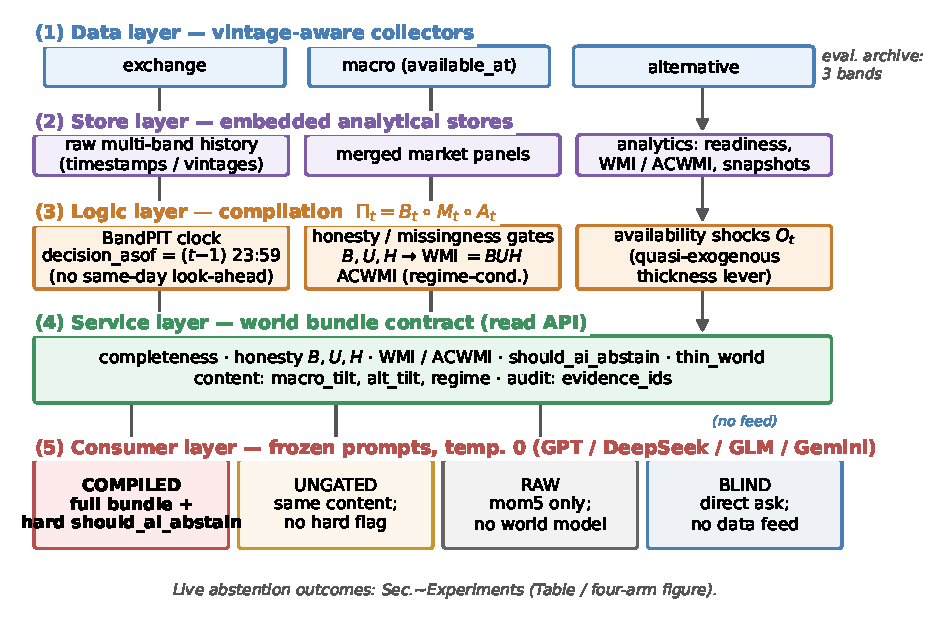
\includegraphics[width=\linewidth]{fig_runtime_architecture.pdf}
  \Description{Layered observation runtime from collectors to world-bundle consumers.}
  \caption{Observation-layer runtime: raw multi-band evidence $\rightarrow$ PIT world bundle $\rightarrow$ Compiled / Ungated / Raw / Blind consumers.}
  \label{fig:pipeline}
\end{figure}

\begin{table}[t]
  \caption{Module map.}
  \label{tab:modules}
  \small
  \begin{tabular}{ll}
    \toprule
    Module & Role \\
    \midrule
    Collectors / stores & Vintage multi-band history \\
    BandPIT compiler & Previous-close \(\Pi_t\), WMI/ACWMI \\
    Bundle builder & Complete / honest / auditable JSON \\
    LLM adapter & OpenAI-compatible chat; temp.\ \(0\) \\
    Eval harness & Four-arm sampling and tables \\
    \bottomrule
  \end{tabular}
\end{table}

\paragraph{Evaluation archive.}
Three public bands: exchange (klines, funding, OI), macro (vintaged risk indices), alternative (stablecoin circulation).
For day \(t\), information is reconstructed at \((t{-}1)\,23{:}59\); payoff is same-day close-to-close return.
Figure~\ref{fig:ready} shows PIT readiness: macro and alternative stay ready; exchange drops later and defines the within-archive thick/thin contrast.
Listing~\ref{lst:bundle} shows a Compiled bundle on an exchange-gap day: two bands ready, low WMI, hard abstain true, evidence IDs binding the view.

\begin{figure}[t]
  \centering
  
\includegraphics[width=0.98\linewidth]{fig_band_readiness.pdf}
  \Description{Band readiness for exchange, macro, and alternative over time.}
  \caption{PIT readiness for the three-band archive (exchange readiness drops later).}
  \label{fig:ready}
\end{figure}

\begin{lstlisting}[caption={Compiled world bundle (compact OOS example).},label={lst:bundle}]
{"date":"2026-05-11","asset":"ADA",
 "decision_asof":"2026-05-10T23:59:00",
 "completeness":{"n_ready":2,"n_missing":1},
 "world_model_index":{"wmi":0.015,
   "should_ai_abstain":true,"thin_world":true},
 "macro_tilt":1.0,"alt_tilt":-1.0,
 "audit":{"evidence_ids":[
   "band:exchange:missing","band:macro:ready"]}}
\end{lstlisting}

\paragraph{Four arms.}
\textbf{Compiled:} full bundle; must abstain when the hard flag is true (the frozen prompt also forbids acting when the world is judged thin).
\textbf{Ungated:} same content and numeric WMI; soft ``you may abstain.''
\textbf{Raw:} \texttt{mom5} only---common thin wiring, not a strongest-agent baseline.
\textbf{Blind:} no feed.
Refuse when \(\mathrm{WMI}<0.2\). On this scarce panel max WMI \({\approx}0.093\), every OOS day is thin under the production gate---a stress test of the valve, not proof the layer never opens.

\paragraph{Prompt difference (only gating).}
Compiled requires abstain when the hard flag is true or the world is thin; Ungated asks the model to judge thinness with no forced policy. Both see the same bundle content. That is intentional: the valve must be enforceable, not hoped for.

\section{Experiments}
\label{sec:exp}

\subsection{Setup}
PIT panel \(\sim\)399 days, 10 liquid names, IS/OOS \(200/200\) days.
Live arms share the same stratified \(100\) OOS asset-days (seed fixed) unless noted; temperature \(0\); four flash/mini vendors in Table~\ref{tab:grounding}.
The no-LLM probe uses \(199\) OOS days after return alignment.

\subsection{RQ1 (primary): Seeing---grounding workflow}
\label{sec:grounding}
If the observation layer works, models should report what the bundle discloses.
On \(50\) OOS asset-days, given Compiled or Raw inputs, each model must list ready bands, missing bands, and \(\mathrm{sign}(\mathrm{macro\_tilt})\), \(\mathrm{sign}(\mathrm{alt\_tilt})\), scored against PIT truth.
Table~\ref{tab:grounding}: Compiled mean ready F1 \(0.97\), missing F1 \(0.97\), tilt-sign accuracy \(0.97\); Raw collapses to \(0.04\), \(0.23\), \(0.19\).
Sufficiency chat alone is weak---models may call a \(3/3\)-ready day ``enough'' while WMI still marks the world thin.
The sharp claim is \emph{verifiability}: only the compiled bundle lets the model state a checkable view of the market.

\begin{table}[t]
  \caption{Grounding ($50$ days): ready / missing / tilt signs. Primary seeing result.}
  \label{tab:grounding}
  \small
  \begin{tabular}{lrrrrrr}
    \toprule
    & \multicolumn{2}{c}{Ready F1} & \multicolumn{2}{c}{Missing F1} & \multicolumn{2}{c}{Tilt-sign} \\
    Model & C & R & C & R & C & R \\
    \midrule
    gpt-5.4-mini & $0.94$ & $0.00$ & $0.94$ & $0.31$ & $0.94$ & $0.20$ \\
    deepseek-v4-flash & $0.98$ & $0.06$ & $0.98$ & $0.20$ & $0.98$ & $0.18$ \\
    glm-5.2 & $0.98$ & $0.09$ & $1.00$ & $0.11$ & $0.98$ & $0.20$ \\
    gemini-3.5-flash-lite & $0.96$ & $0.03$ & $0.96$ & $0.30$ & $0.96$ & $0.18$ \\
    \midrule
    Mean & $0.97$ & $0.04$ & $0.97$ & $0.23$ & $0.97$ & $0.19$ \\
    \bottomrule
  \end{tabular}
\end{table}

\subsection{RQ2 (safety valve): Hard refuse when the view is thin}
\label{sec:gate}
Seeing is not enough if thin worlds still drive action.
Table~\ref{tab:llm} and Figure~\ref{fig:und}: on the same \(100\) days, Compiled abstains on every thin day (\(1.0\)); Ungated soft-judges at mean \(0.68\) (Gemini \(0.43\)); Raw over-trades (abstain as low as \(0.04\); Table~\ref{tab:mix}); Blind abstains \(1.0\) with no feed.
The costly failure mode is the middle case: half-baked Raw context makes models act and lose.
Mean \(\Delta\)CE (Compiled$-$Raw) \({+}1.07\) is avoided loss under the valve, not an alpha claim.
Full-OOS (\(n{=}2000\), all thin) reproduces Compiled \(1.0\) and Ungated mean \({\approx}0.56\).

\begin{table}[t]
  \caption{Thin-world abstention on identical $100$ OOS days (Wilson 95\% CIs). Blind abstains $1.0$. $\Delta$CE $=$ avoided loss.}
  \label{tab:llm}
  \small
  \begin{tabular}{lrrrr}
    \toprule
    Model & Thin C & Thin U {\scriptsize[CI]} & Abs.\ R {\scriptsize[CI]} & \(\Delta\)CE \\
    \midrule
    gpt-5.4-mini & $1.00$ & $0.63$ {\scriptsize[.53,.72]} & $0.04$ {\scriptsize[.02,.10]} & $+0.73$ \\
    deepseek-v4-flash & $1.00$ & $0.81$ {\scriptsize[.72,.87]} & $0.75$ {\scriptsize[.66,.82]} & $+1.22$ \\
    glm-5.2 & $1.00$ & $0.86$ {\scriptsize[.78,.91]} & $0.11$ {\scriptsize[.06,.19]} & $+1.04$ \\
    gemini-3.5-flash-lite & $1.00$ & $0.43$ {\scriptsize[.34,.53]} & $0.07$ {\scriptsize[.03,.14]} & $+1.30$ \\
    \midrule
    Mean & $1.00$ & $0.68$ & --- & $+1.07$ \\
    \bottomrule
  \end{tabular}
\end{table}

\begin{figure}[t]
  \centering
  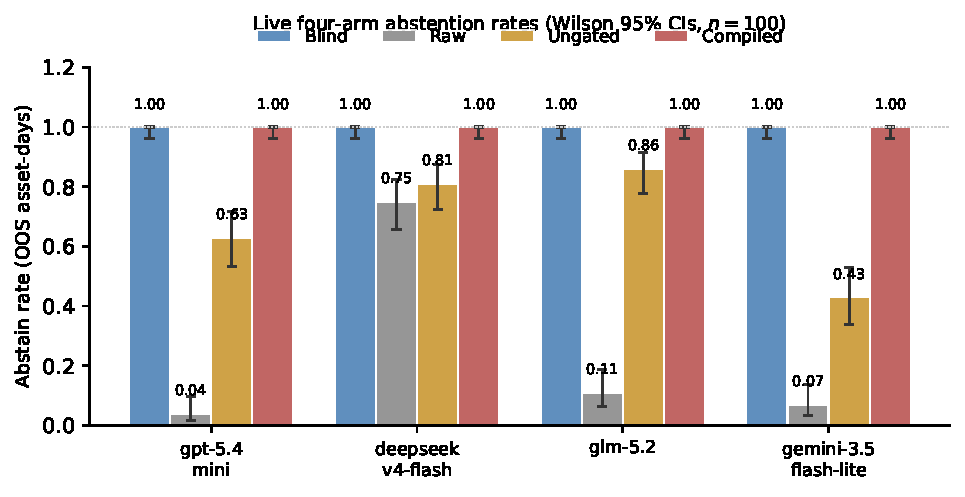
\includegraphics[width=\linewidth]{fig_four_arm_ladder.pdf}
  \Description{Four-arm abstain rates with Wilson error bars.}
  \caption{Safety-valve ranking: Blind refuses; Raw over-trades; Ungated is unstable; Compiled enforces the hard gate.}
  \label{fig:und}
\end{figure}

\begin{table}[t]
  \caption{Raw action mix ($100$ days): half-baked context drives directional mass.}
  \label{tab:mix}
  \small
  \begin{tabular}{lrrrr}
    \toprule
    Model & Abs. & Bull. & Bear. & Neut. \\
    \midrule
    gpt-5.4-mini & $0.04$ & $0.28$ & $0.38$ & $0.30$ \\
    deepseek-v4-flash & $0.75$ & $0.14$ & $0.04$ & $0.07$ \\
    glm-5.2 & $0.11$ & $0.40$ & $0.48$ & $0.01$ \\
    gemini-3.5-flash-lite & $0.07$ & $0.44$ & $0.49$ & $0.00$ \\
    \bottomrule
  \end{tabular}
\end{table}

\paragraph{Scarce-panel note (once).}
Production Compiled never opens at WMI \({<}0.2\) on this archive.
On band-thick / open-slice days (\(3/3\) ready \(\equiv\mathrm{WMI}\ge 0.05\); \(n{=}1224\)), Ungated keeps content without the hard boolean: four-vendor mean CE \({\approx}{+}0.29\); block-bootstrap mean \({\approx}{+}0.31\) with CIs including zero---a content lower bound, \emph{not} Compiled-open trading (the prompt's thinness clause can still force abstain).
Denser vintages can raise the WMI floor without changing layer semantics.

\subsection{RQ3 (secondary): Nonempty bundle fields}
\label{sec:econ}
A transparent no-LLM rule adds vintaged \(\mathrm{macro\_tilt}\) / \(\mathrm{alt\_tilt}\) to return inputs shared with momentum.
OOS: Sharpe \(0.764\) / CE \({+}0.130\) vs.\ momentum (\(0.096\), \(-0.206\)) and buy-and-hold (\(-1.404\), \(-1.163\)); \(\Delta\mathrm{CE}{=}0.334\) (\(p{=}0.034\); Figure~\ref{fig:econ}).
LOBO attributes the gap to band content; a long non-vintaged audit shows no edge.
This supports nonempty fields in the observation layer, not an LLM leaderboard.

\begin{figure}[t]
  \centering
  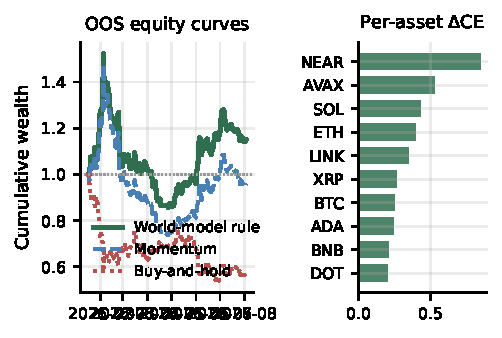
\includegraphics[width=\linewidth]{fig_oos_economics.pdf}
  \Description{Equity curves and per-asset delta CE for the no-LLM content rule.}
  \caption{Secondary content probe (no LLM): compiled tilts beat momentum; $\Delta$CE positive for every asset.}
  \label{fig:econ}
\end{figure}

\subsection{Discussion}
\paragraph{What carries the paper.}
(i)~\emph{The bundle is legible} (RQ1).
(ii)~\emph{Thin views must not drive action}---soft text fails; the hard valve works (RQ2).
(iii)~\emph{Fields are nonempty} under a no-LLM probe (RQ3).
Relative to FinMem~/FinAgent and ICAIF agent stacks~\cite{yu2023finmem,zhang2024finagent,choi2025finagentbench,shen2025finsearch,sun2025finresearchbench,duan2025factormad}, we contribute the observation layer those systems assume.

\paragraph{Threats.}
Compiled thin abstention is quality-gate obedience by design.
The archive is scarce; open-slice Ungated is not Compiled-open; CE bootstrap CIs include zero.
Vendors are flash/mini at temperature \(0\); Raw is common \texttt{mom5} wiring for the four-arm ladder, not dominance over tool agents.
Decision/execution stacks can sit on top once denser bands lift WMI above the scarce floor.

\section{Conclusion}
\label{sec:conc}

Public LLMs need a market they can see before they decide.
We contribute an observation layer that compiles asynchronous crypto evidence into a consumable PIT world bundle, and forces abstention when the view is too thin.
Live, models recover ready/missing/tilt at \({\approx}0.97\) under Compiled vs.\ Raw collapse; the hard valve abstains \(1.0\) on thin days where soft judgment does not.
Compile so models can see; refuse when they must not act.

\begin{acks}
Omitted for anonymous review.
\end{acks}

\bibliographystyle{ACM-Reference-Format}
\bibliography{refs}

\end{document}
